\documentclass[a4paper,11pt]{exam}
\printanswers % pour imprimer les réponses (corrigé)
%\noprintanswers % Pour ne pas imprimer les réponses (énoncé)
\addpoints % Pour compter les points
% \noaddpoints % pour ne pas compter les points
%\qformat{\textbf{\thequestion ) } }
\qformat{\textbf{\thequestion )} (\thepoints) \\} % Pour définir le style des questions (facultatif)
\usepackage{color} % définit une nouvelle couleur
\shadedsolutions % définit le style des réponses
% \framedsolutions % définit le style des réponses
\definecolor{SolutionColor}{rgb}{0.8,0.9,1} % bleu ciel
\renewcommand{\solutiontitle}{\noindent\textbf{Solution:}\par\noindent} % Définit le titre des solutions




\makeatletter

\def\maketitle{{\centering%
	\par{\huge\textbf{\@title}}%
	\par{\@date}%
	\par}}

\makeatother

\lhead{NOM Pr\'enom :}
\rhead{\textbf{Les r\'eponses doivent \^etre justifi\'ees}}
\cfoot{\thepage / \pageref{LastPage}}


%\usepackage{../../pas-math}
%\usepackage{../../moncours}


%\usepackage{pas-cours}
%-------------------------------------------------------------------------------
%          -Packages nécessaires pour écrire en Français et en UTF8-
%-------------------------------------------------------------------------------
\usepackage[utf8]{inputenc}
\usepackage[frenchb]{babel}
\usepackage[T1]{fontenc}
\usepackage{lmodern}
\usepackage{textcomp}



%-------------------------------------------------------------------------------

%-------------------------------------------------------------------------------
%                          -Outils de mise en forme-
%-------------------------------------------------------------------------------
\usepackage{hyperref}
\hypersetup{pdfstartview=XYZ}
%\usepackage{enumerate}
\usepackage{graphicx}
\usepackage{multicol}
\usepackage{tabularx}
\usepackage{multirow}


\usepackage{anysize} %%pour pouvoir mettre les marges qu'on veut
%\marginsize{2.5cm}{2.5cm}{2.5cm}{2.5cm}

\usepackage{indentfirst} %%pour que les premier paragraphes soient aussi indentés
\usepackage{verbatim}
\usepackage{enumitem}
\usepackage[usenames,dvipsnames,svgnames,table]{xcolor}

\usepackage{variations}

%-------------------------------------------------------------------------------


%-------------------------------------------------------------------------------
%                  -Nécessaires pour écrire des mathématiques-
%-------------------------------------------------------------------------------
\usepackage{amsfonts}
\usepackage{amssymb}
\usepackage{amsmath}
\usepackage{amsthm}
\usepackage{tikz}
\usepackage{xlop}
%-------------------------------------------------------------------------------



%-------------------------------------------------------------------------------


%-------------------------------------------------------------------------------
%                    - Mise en forme avancée
%-------------------------------------------------------------------------------

\usepackage{ifthen}
\usepackage{ifmtarg}


\newcommand{\ifTrue}[2]{\ifthenelse{\equal{#1}{true}}{#2}{$\qquad \qquad$}}

%-------------------------------------------------------------------------------

%-------------------------------------------------------------------------------
%                     -Mise en forme d'exercices-
%-------------------------------------------------------------------------------
%\newtheoremstyle{exostyle}
%{\topsep}% espace avant
%{\topsep}% espace apres
%{}% Police utilisee par le style de thm
%{}% Indentation (vide = aucune, \parindent = indentation paragraphe)
%{\bfseries}% Police du titre de thm
%{.}% Signe de ponctuation apres le titre du thm
%{ }% Espace apres le titre du thm (\newline = linebreak)
%{\thmname{#1}\thmnumber{ #2}\thmnote{. \normalfont{\textit{#3}}}}% composants du titre du thm : \thmname = nom du thm, \thmnumber = numéro du thm, \thmnote = sous-titre du thm

%\theoremstyle{exostyle}
%\newtheorem{exercice}{Exercice}
%
%\newenvironment{questions}{
%\begin{enumerate}[\hspace{12pt}\bfseries\itshape a.]}{\end{enumerate}
%} %mettre un 1 à la place du a si on veut des numéros au lieu de lettres pour les questions 
%-------------------------------------------------------------------------------

%-------------------------------------------------------------------------------
%                    - Mise en forme de tableaux -
%-------------------------------------------------------------------------------

\renewcommand{\arraystretch}{1.7}

\setlength{\tabcolsep}{1.2cm}

%-------------------------------------------------------------------------------



%-------------------------------------------------------------------------------
%                    - Racourcis d'écriture -
%-------------------------------------------------------------------------------

% Angles orientés (couples de vecteurs)
\newcommand{\aopp}[2]{(\vec{#1}, \vec{#2})} %Les deuc vecteurs sont positifs
\newcommand{\aopn}[2]{(\vec{#1}, -\vec{#2})} %Le second vecteur est négatif
\newcommand{\aonp}[2]{(-\vec{#1}, \vec{#2})} %Le premier vecteur est négatif
\newcommand{\aonn}[2]{(-\vec{#1}, -\vec{#2})} %Les deux vecteurs sont négatifs

%Ensembles mathématiques
\newcommand{\naturels}{\mathbb{N}} %Nombres naturels
\newcommand{\relatifs}{\mathbb{Z}} %Nombres relatifs
\newcommand{\rationnels}{\mathbb{Q}} %Nombres rationnels
\newcommand{\reels}{\mathbb{R}} %Nombres réels
\newcommand{\complexes}{\mathbb{C}} %Nombres complexes


%Intégration des parenthèses aux cosinus
\newcommand{\cosP}[1]{\cos\left(#1\right)}
\newcommand{\sinP}[1]{\sin\left(#1\right)}


%Probas stats
\newcommand{\stat}{statistique}
\newcommand{\stats}{statistiques}
%-------------------------------------------------------------------------------

%-------------------------------------------------------------------------------
%                    - Mise en page -
%-------------------------------------------------------------------------------

\newcommand{\twoCol}[1]{\begin{multicols}{2}#1\end{multicols}}


\setenumerate[1]{font=\bfseries,label=\textit{\alph*})}
\setenumerate[2]{font=\bfseries,label=\arabic*)}


%-------------------------------------------------------------------------------
%                    - Elements cours -
%-------------------------------------------------------------------------------





%\usepackage{fullpage}
\author{\ }
\date{18 Novembre 2019}
\title{$5^e G$ : DS num\'ero 2}


\begin{document}
%	\usepackage{fancyhdr}
%	
%	\pagestyle{fancy}
%	\fancyhf{}
	%\rhead{Share\LaTeX}

	\maketitle
	
\begin{center}
	\textbf{Calculatrice interdite}
\end{center}

%
%{ (Ch2)} :   (sur une feuille de papier, avec des objets, à l’aide de logiciels), chercher des exemples ou des contre-exemples;
%\item \kw{Raisonner (Ra3)} :   ;
%\item \kw{Communiquer (Co2)} :  expliquer à l’oral ou à l’écrit sa démarche ou son raisonnement; 
\begin{small}
	\begin{center}
		\begin{tabular}{|@{\ }l@{\ }|@{\ }c@{\ }|@{\ }c@{\ }|@{\ }c@{\ }|@{\ }c@{\ }|}
			\hline
			\textbf{Compétence} & \textbf{MI} & \textbf{MF} & \textbf{MS} & \textbf{TBM} \\
			\hline
			\textbf{Chercher} (observer, questionner, manipuler, expérimenter) (Ex 3)&  \ \ & \ \ & \ \ & \ \  \\
			\hline	
			\textbf{Raisonner} (utiliser un raisonnement logique pour parvenir à une conclusion) (Ex 5)& \ \ & \ \ &  \ \  & \ \ \\
			\hline
			\textbf{Communiquer} (Expliquer sa démarche, son raisonnement ) &  \ \ & \ \ & \ \ & \ \  \\
			\hline
		\end{tabular}
	\end{center}
\end{small}	

	
	
\section{Figures symétriques (3 points)}

\begin{questions}
	\question[3] Entourer les couples de figures qui semblent être symétriques par rapport à un point.
	
	\begin{center}
		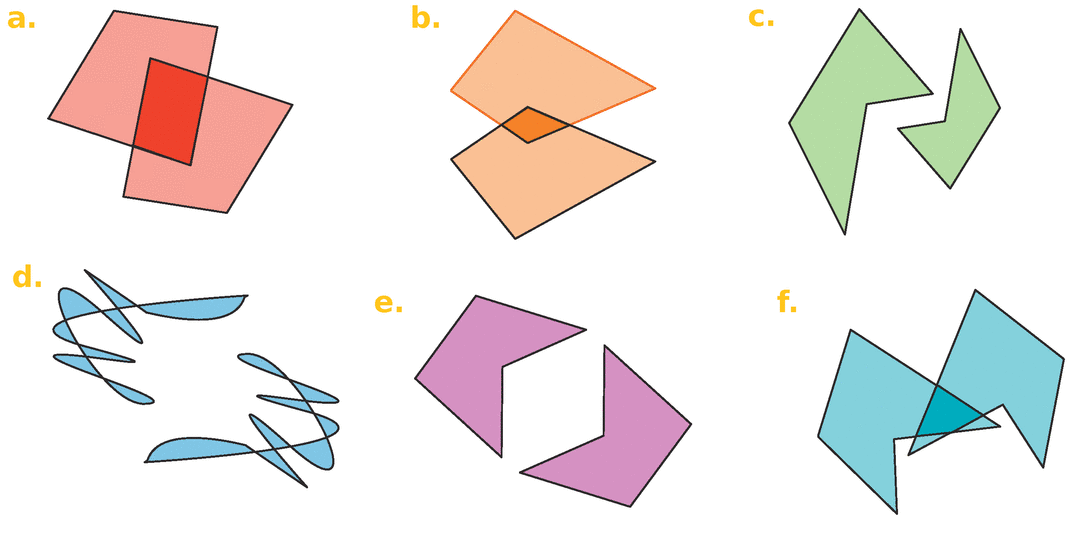
\includegraphics[scale=0.4]{img/figures}
	\end{center} 

	\begin{solution}
		\begin{center}
			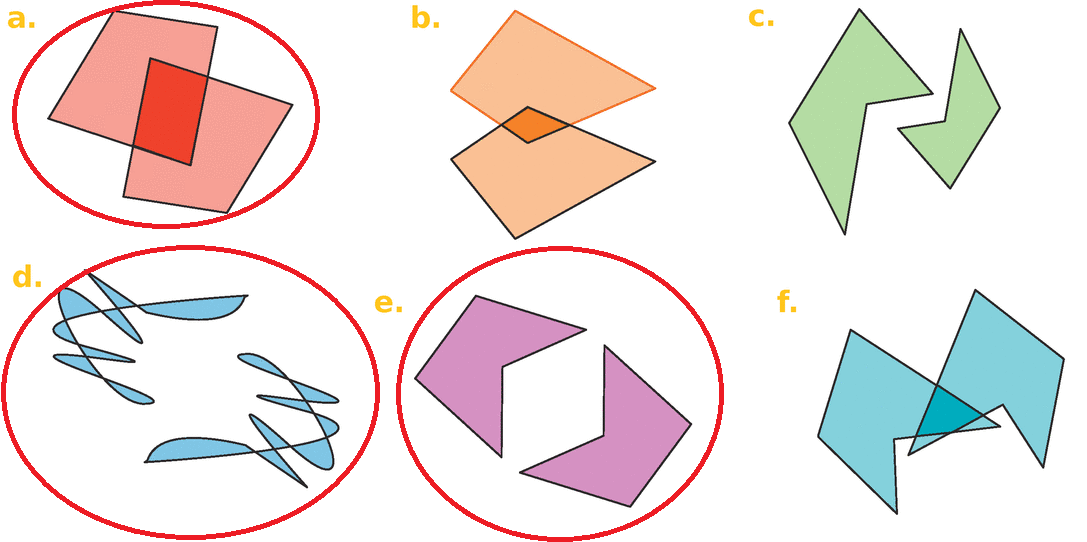
\includegraphics[scale=0.4]{img/figures_corr}
		\end{center} 
	\end{solution}
\end{questions}


	

\newpage

\section{Pavage (3 poinst)}

\begin{questions}
	\question[3] Dans cette image, mettre en évidence deux axes de symétrie et deux centres de symétrie.
\end{questions}


\begin{center}
	
\includegraphics[scale=0.5]{img/anges}
\end{center}

\newpage

\section{Construction (6 points)}

\begin{questions}
	\question[3] Construire en vraie grandeur la figure ci-dessous.
	\begin{center}
		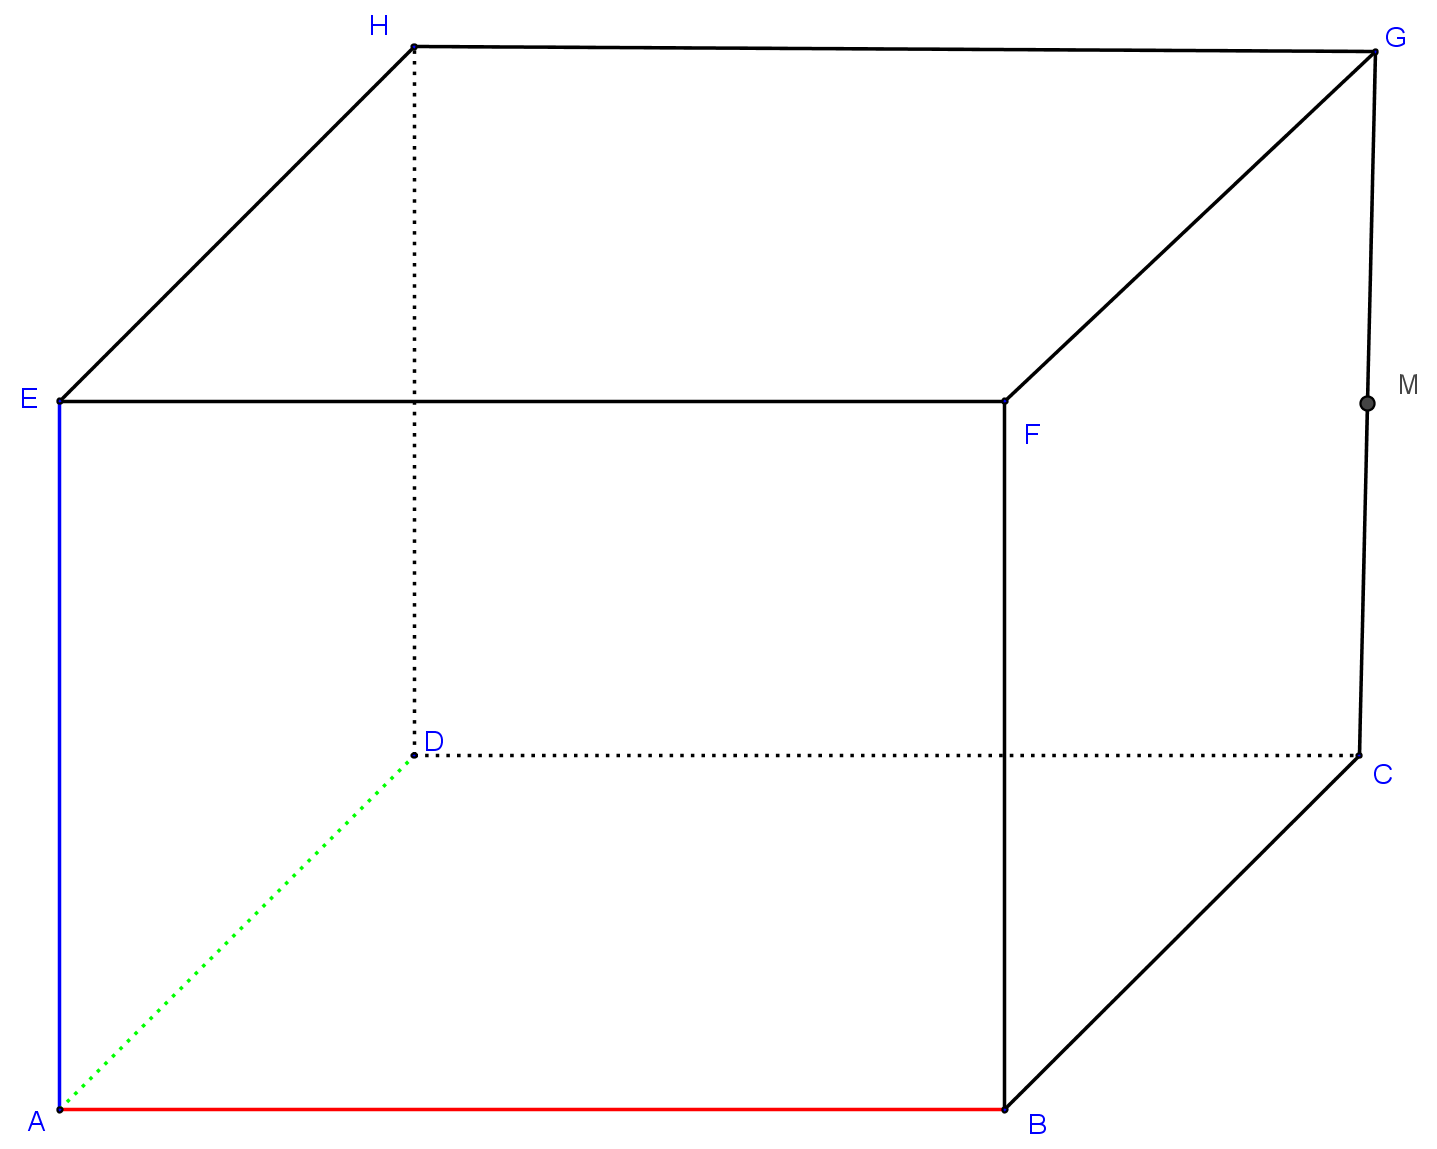
\includegraphics[scale=0.7]{img/figure}
	\end{center}

	\question 
		\begin{parts}
			\part[1] Sur votre figure, les points A, B et C semblent-t-ils alignés.
			
			\part[2] Le sont-ils vraiment ? Justifier votre réponse.
		\end{parts}
\end{questions}

\newpage
\section{Spectacle (3 points)}

Pour le spectacle de fin d'année, la maîtresse a placé 7 élèves de ma classe de CE2 comme sur le schéma ci-dessous.

\begin{center}
	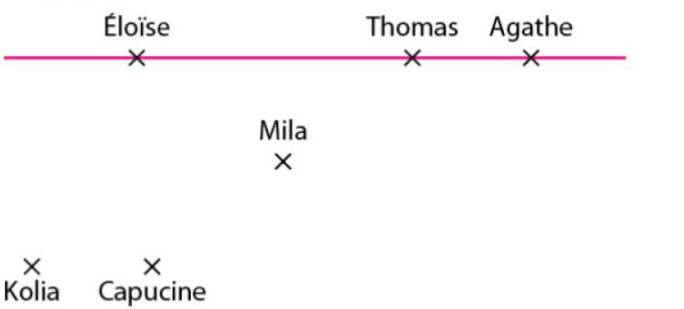
\includegraphics[scale=0.5]{img/spectacle}
\end{center}

Elle veut que la position des élèves soit symétrique par rapport à celle de Mila.

\begin{questions}
	\question[1\half] En utilisant uniquement une règle non graduée, déterminer la position d'Eneko, le dernier élève à ne pas avoir encore été placé. Laisser apparents les traits de construction.
	
	\begin{solution}
		\begin{center}
			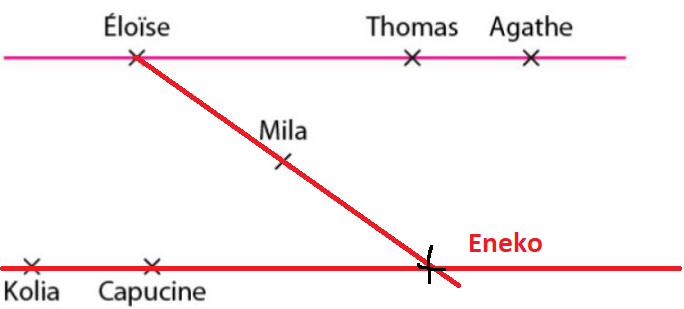
\includegraphics[scale=0.5]{img/spectacle_corr}
		\end{center}
	\end{solution}
	
	\question[1\half] Quelle propriété permet de répondre à la question ?
	\begin{solution}
		On sait que \'Eloïse, Thomas et Agathe sont alignés,
		or le symétrique d'une droite par rapport à un point est une autre droite. 
		Donc Kolia, Capucine et Thomas seront aussi alignés.
	\end{solution}
\end{questions}

\newpage

\section{Tabouret (4 poins)}

\begin{multicols}{2}
	Guillaume a déplié sont tabouret. L'assise (le segment $[AB]$) mesure 65 cm.

\begin{questions}
	
	\question[2] L'assise est-elle parallèle au sol ? Le démonter.
	
	\begin{solution}
		On sait que $(AB)$ et $(DE)$ sont symétriques par rapport à $C$.
		Or le symétrique d'une droite par rapport à un point est une droite parallèle à la première.
		Donc $(AB)$ // $(DE)$.
		
		L'assise est du tabouret est parallèle au sol.
	\end{solution}

	\question[2] Quel est l'écartement entre les pieds ? Le démontrer.
	\begin{solution}
		On sait que $C$ est le milieu de $[AD]$ et de $[BE]$, donc $C$ est le symétrique de $A$ et $E$ celui de $B$ par rapport à $C$.\\
		
		On sait que $[AB]$ et $[DE]$ sont symétriques par rapport à $C$.
		Or la symétrie conserve les longueurs.
		Donc $AB$ = $DE$.
		
		L'écartement entre les pieds est de 65 cm.
		
	\end{solution}
	
	
\end{questions}

\begin{center}
	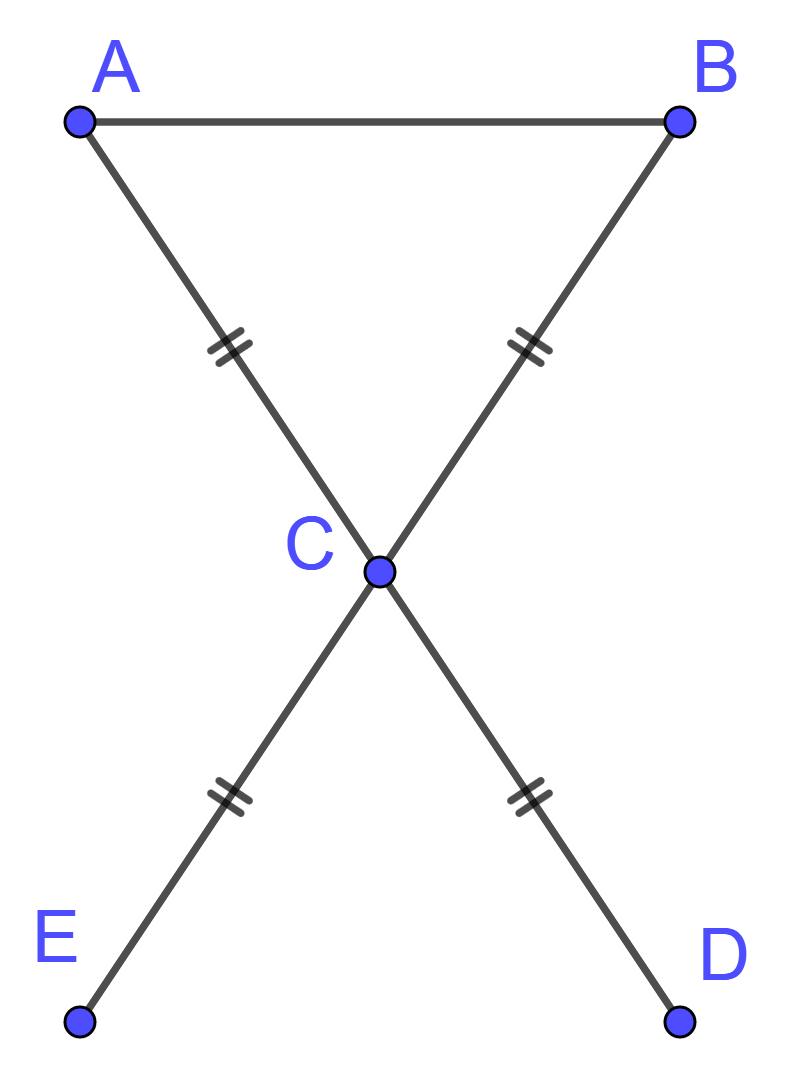
\includegraphics[scale=0.13]{img/tabouret}
\end{center}
	
	
\end{multicols}

\section{Bonus : Figure incomplète (3 points) }

$ABCD$ est un carré qui a été en partie effacé. On veut tracer son symétrique par rapport au point $O$.

\begin{questions}
	\question[1] Sans compléter le carré $ABCD$, construire $A'B'C'D'$, son symétrique par raport à $O$.
	
	\question[2] \'Ecrire un programme de construction pour $A'B'C'D'$.
\end{questions}

\begin{center}
	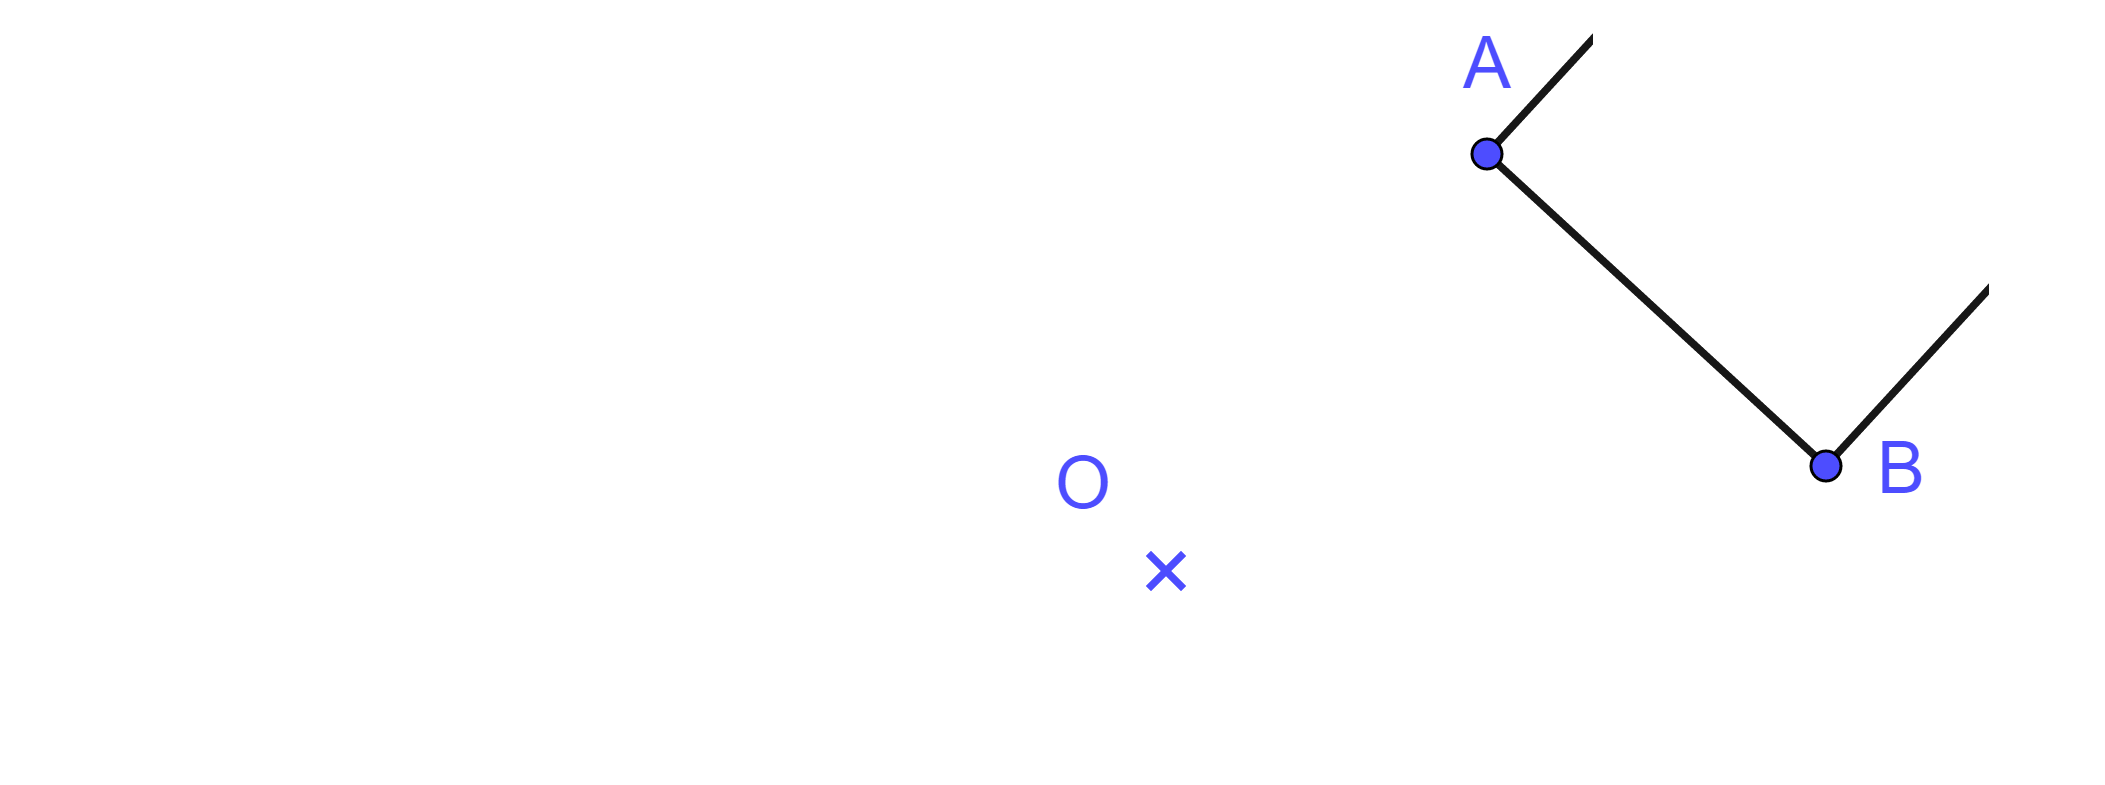
\includegraphics[scale=0.3]{img/carre}
\end{center}
\label{LastPage}

\end{document}